\section{Pendahuluan}
\subsection{Latar Belakang}
VPN atau Jaringan Pribadi Virtual (Virtual Private Network) membuat koneksi jaringan privat di
antara beberapa perangkat melalui internet. VPN digunakan untuk mentransmisikan data secara aman
dan anonim melalui jaringan publik. VPN bekerja dengan cara menyembunyikan alamat IP pengguna
dan mengenkripsi data sehingga tidak dapat dibaca oleh siapa pun yang tidak berwenang untuk
menerimanya.\\\\
Salah satu service yang biasa digunakan untuk membangun sebuah jaringan VPN adalah Point to
Point Tunnel Protocol (PPTP). Sebuah koneksi PPTP terdiri dari Server dan Client.
Mikrotik RouterOS bisa difungsikan baik sebagai server maupun client atau bahkan diaktifkan
keduanya bersama dalam satu mesin yang sama. Feature ini sudah termasuk dalam package PPP
sehingga anda perlu cek di menu system package apakah paket tersebut sudah ada di router atau
belum. Fungsi PPTP Client juga sudah ada di hampir semua OS, sehingga kita bisa menggunakan
Laptop/PC sebagai PPTP Client.\\\\
Biasanya PPTP ini digunakan untuk jaringan yang sudah melewati multihop router (Routed Network).
Jika anda ingin menggunakan PPTP pastikan di Router anda tidak ada rule yang melakukan blocking
terhadap protocol TCP 1723 dan IP Protocol 47/GRE karena service PPTP menggunakan protocol
tersebut.

\subsection{Maksud dan Tujuan}
Mengetahui cara menggunakan dan mengkonfigurasi VPN PPTP pada router mikrotik.

\subsection{Hasil yang diharapkan}
Memahami penerapan dan penghubungan jaringan dengan menerapkan PPTP dengan VPN

%===========================================================%
\section{Tugas Pendahuluan}
\begin{center}
	\colorbox{cyan!30}{\parbox{0.8\linewidth}{
    \begin{enumerate}
        \item Apa itu PPTP dan bagaimana cara kerjanya?
        \item Apa kelebihan dan kekurangan dari penggunaan PPTP dibandingkan protokol VPN lainnya seperti L2TP atau OpenVPN?
    \end{enumerate}}}
\end{center}

%===========================================================%
\section{Alat dan Bahan}
\begin{itemize}[label=$\bullet$, itemsep=-1pt, leftmargin=*]
	\item 2 buah Cloud Core Router
	\item 3 Kabel UTP (LAN)
	\item 2 buah Laptop
	\item Software Winbox
\end{itemize}

%===========================================================%
\section{Jangka Waktu Pelaksanaan}
Pemahaman dan konfigurasi 1 jam.

%===========================================================%
\section{Penjelasan dan Tahapan Konfigurasi}

%======================PERCOBAAN 1==========================%
\begin{center}
    \textbf{Konfigurasi PC 1}
    \begin{enumerate}
        \item Buka aplikasi Winbox pada PC dan lakukan hubungkan ke Router. Pastikan Login terisi “admin”, Klik Neighbors > Klik Refresh > Pilih Router yang ingin disambungkan > Klik Connect.
        \begin{figure}[H]
			\centering
			\includegraphics[width=0.5\linewidth]{P4/img/pc1/Step 1.png}
			\caption{Step 1}
			\label{fig:Step 1(PC 1)}
		\end{figure}
        \item Jadikan Router menjadi DHCP Client agar bisa mendapat IP address dari Internet ITS. IP > Klik DHCP Client > Tambahkan DHCP Client > Pilih interface yang terhubung dengan Internet (ether2)> Klik Apply > Klik OK. Kita bisa memastikan koneksi ke internet dengan cara melakukan tes ping ke alamat IP 8.8.8.8
        \begin{figure}[H]
			\centering
			\includegraphics[width=0.5\linewidth]{P4/img/pc1/Step 2.1.png}
			\caption{Step 2.1}
			\label{fig:Step 2.1(PC 1)}
        \end{figure}
        \begin{figure}[H]
			\centering
			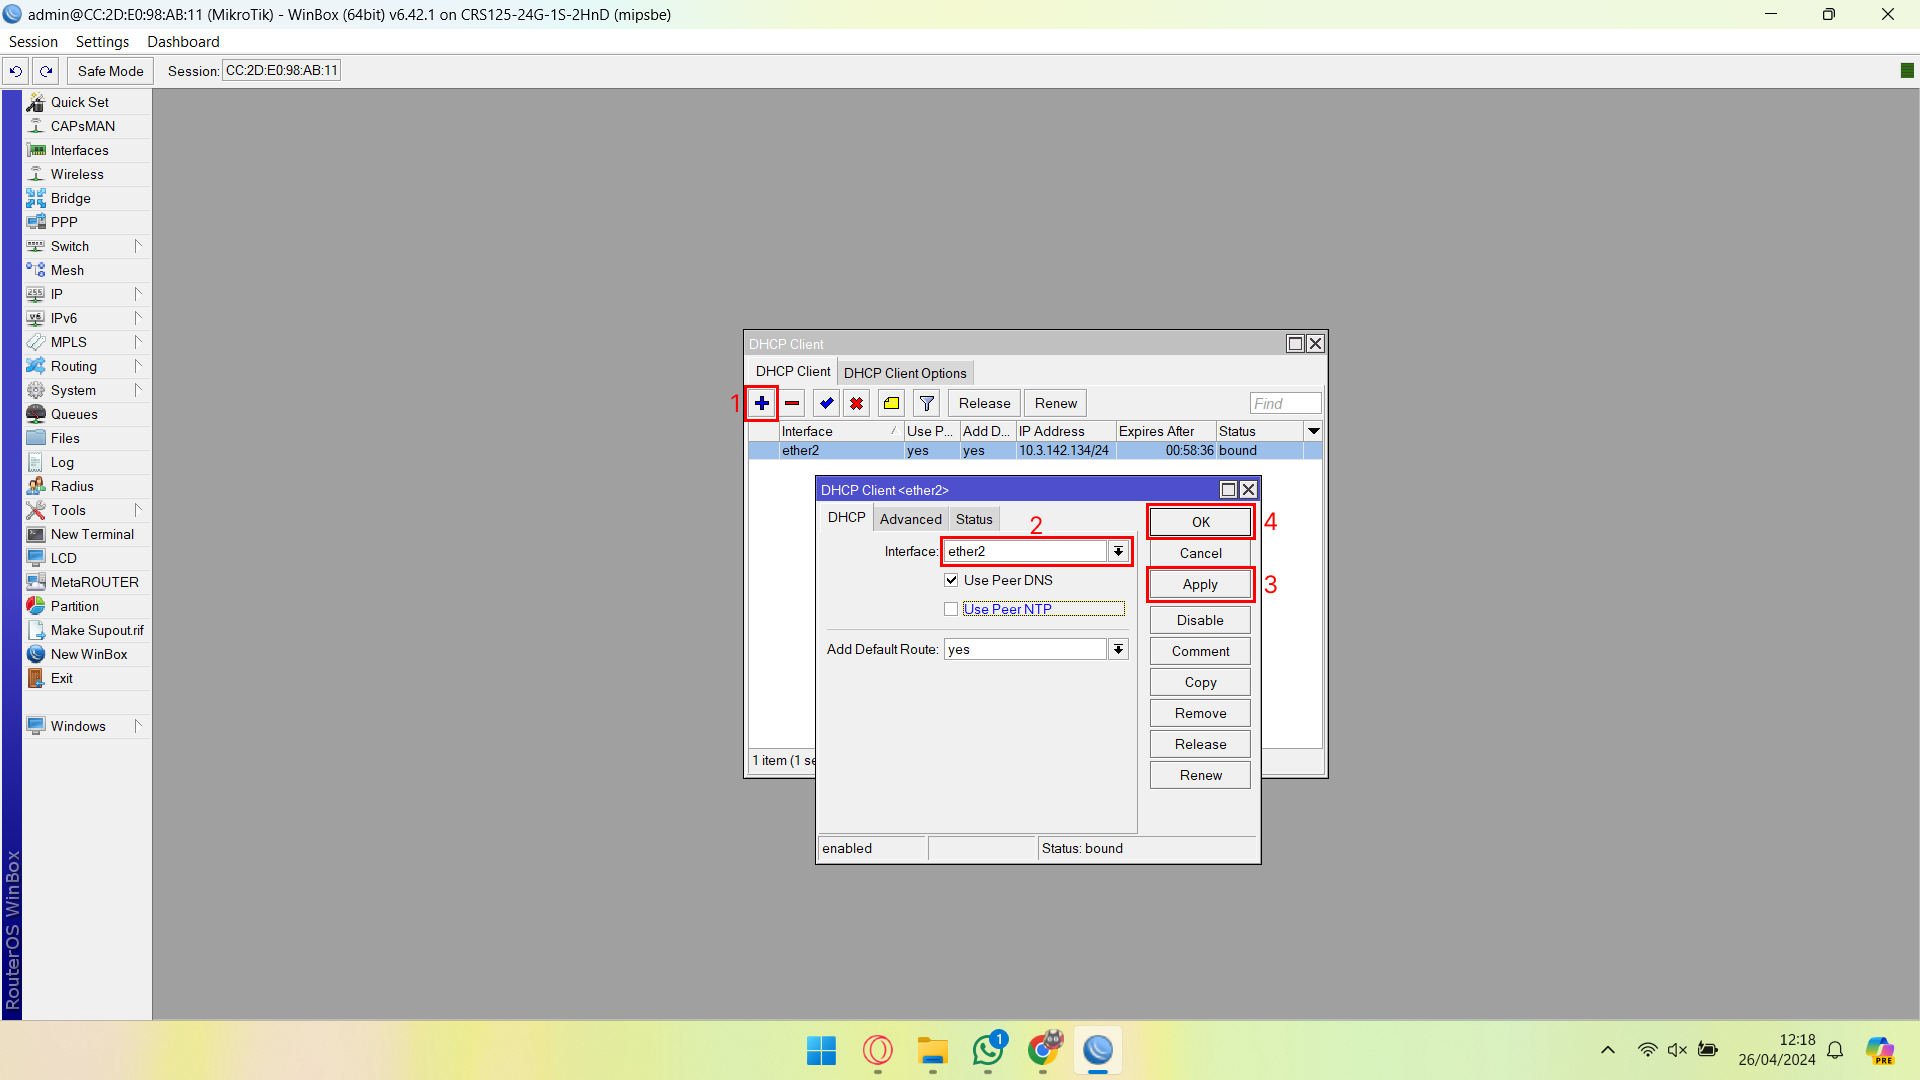
\includegraphics[width=0.8\linewidth]{P4/img/pc1/Step 2.2.png}
			\caption{Step 2.2}
			\label{fig:Step 2.2(PC 1)}
		\end{figure}
        \item Buat IP address baru pada Router 1 untuk menghubungkan PC 1 dengan Router 1. Tambahkan IP address > Isi address > Pilih Interface yang terhubung ke PC (ether4) > Klik Apply > Klik OK.
        \begin{figure}[H]
			\centering
			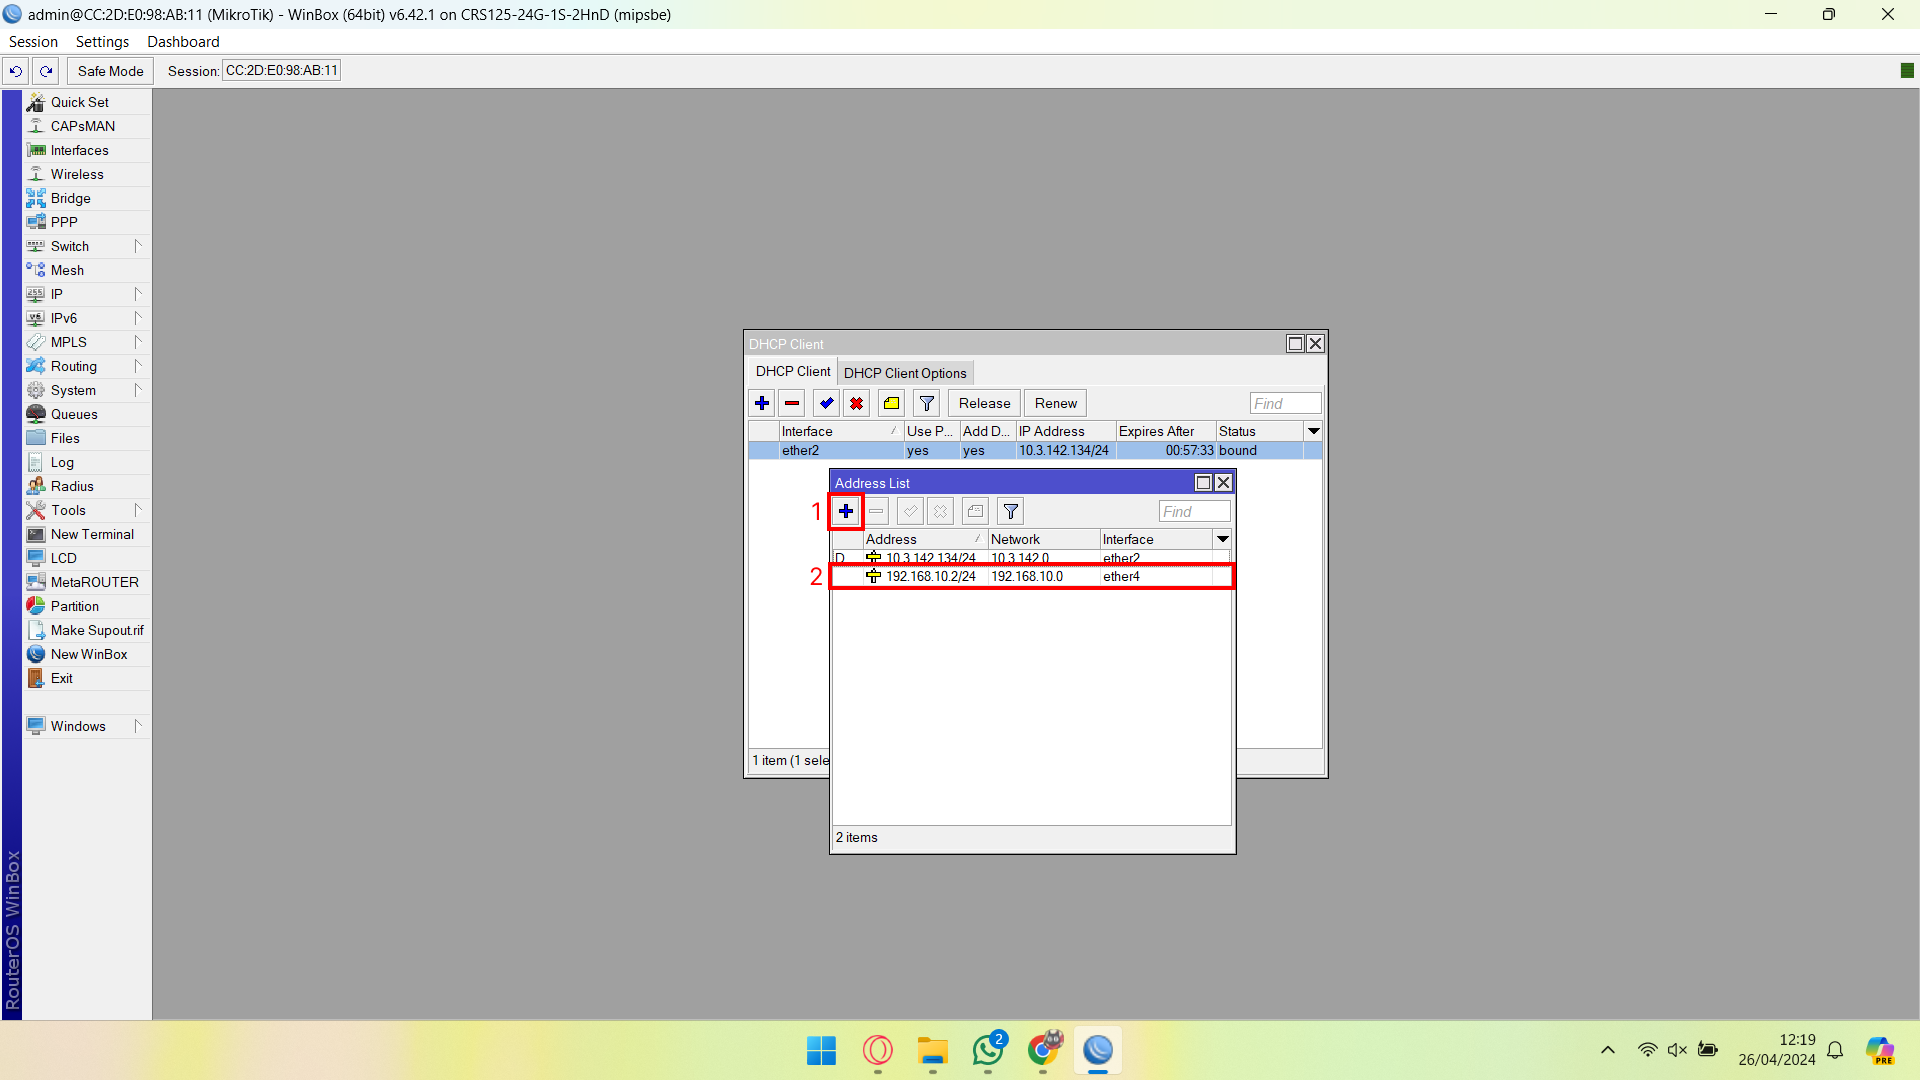
\includegraphics[width=0.8\linewidth]{P4/img/pc1/Step 3.png}
			\caption{Step 3}
			\label{fig:Step 3(PC 1)}
		\end{figure}
        \item Atur IP pada PC 1 dengan mengubah pengaturan pada setting ethernet. Ubah IP perangkat yang otomatis menjadi manual, pastikan IP PC 1 masih satu jaringan dengan IP lokal yang diinginkan, isi Gateway dengan IP address Router 1 yang tersambung dengan PC 1. Berikan IP address yang berbeda dengan contoh yang ada di modul.
        \begin{figure}[H]
			\centering
			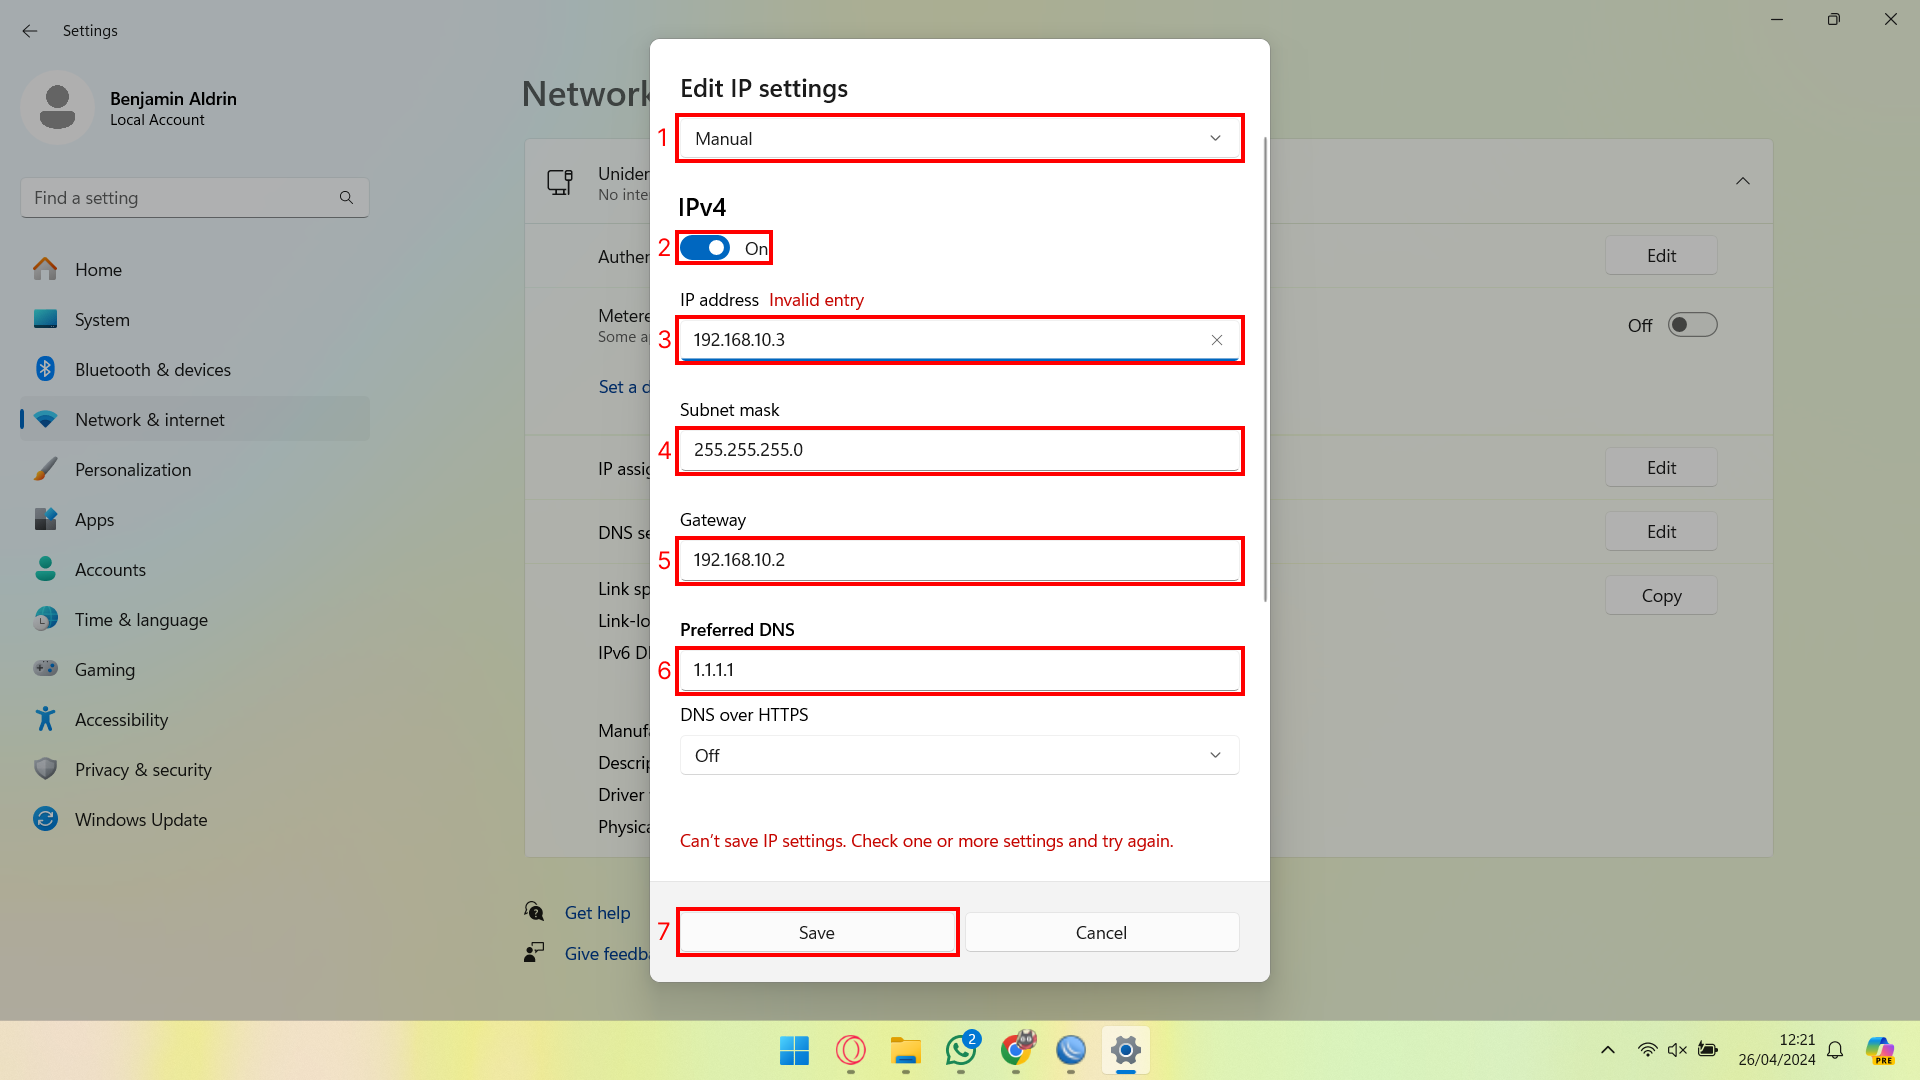
\includegraphics[width=0.8\linewidth]{P4/img/pc1/Step 4.png}
			\caption{Step 4}
			\label{fig:Step 4(PC 1)}
		\end{figure}
        \item Buat PPTP untuk client pada tab Secret, dengan konfigurasi Nama “PPTP”, Password “123456”, Service “pptp”, Profile “default”. Local Address adalah IP address tunnel pada sisi server, diisi dengan “10.10.10.2”. Remote Address adalah IP yang akan Client dapatkan, diisi dengan “10.10.10.3”. Pastikan Local Address dan Remote Address berada pada satu jaringan yang sama.
        \begin{figure}[H]
			\centering
			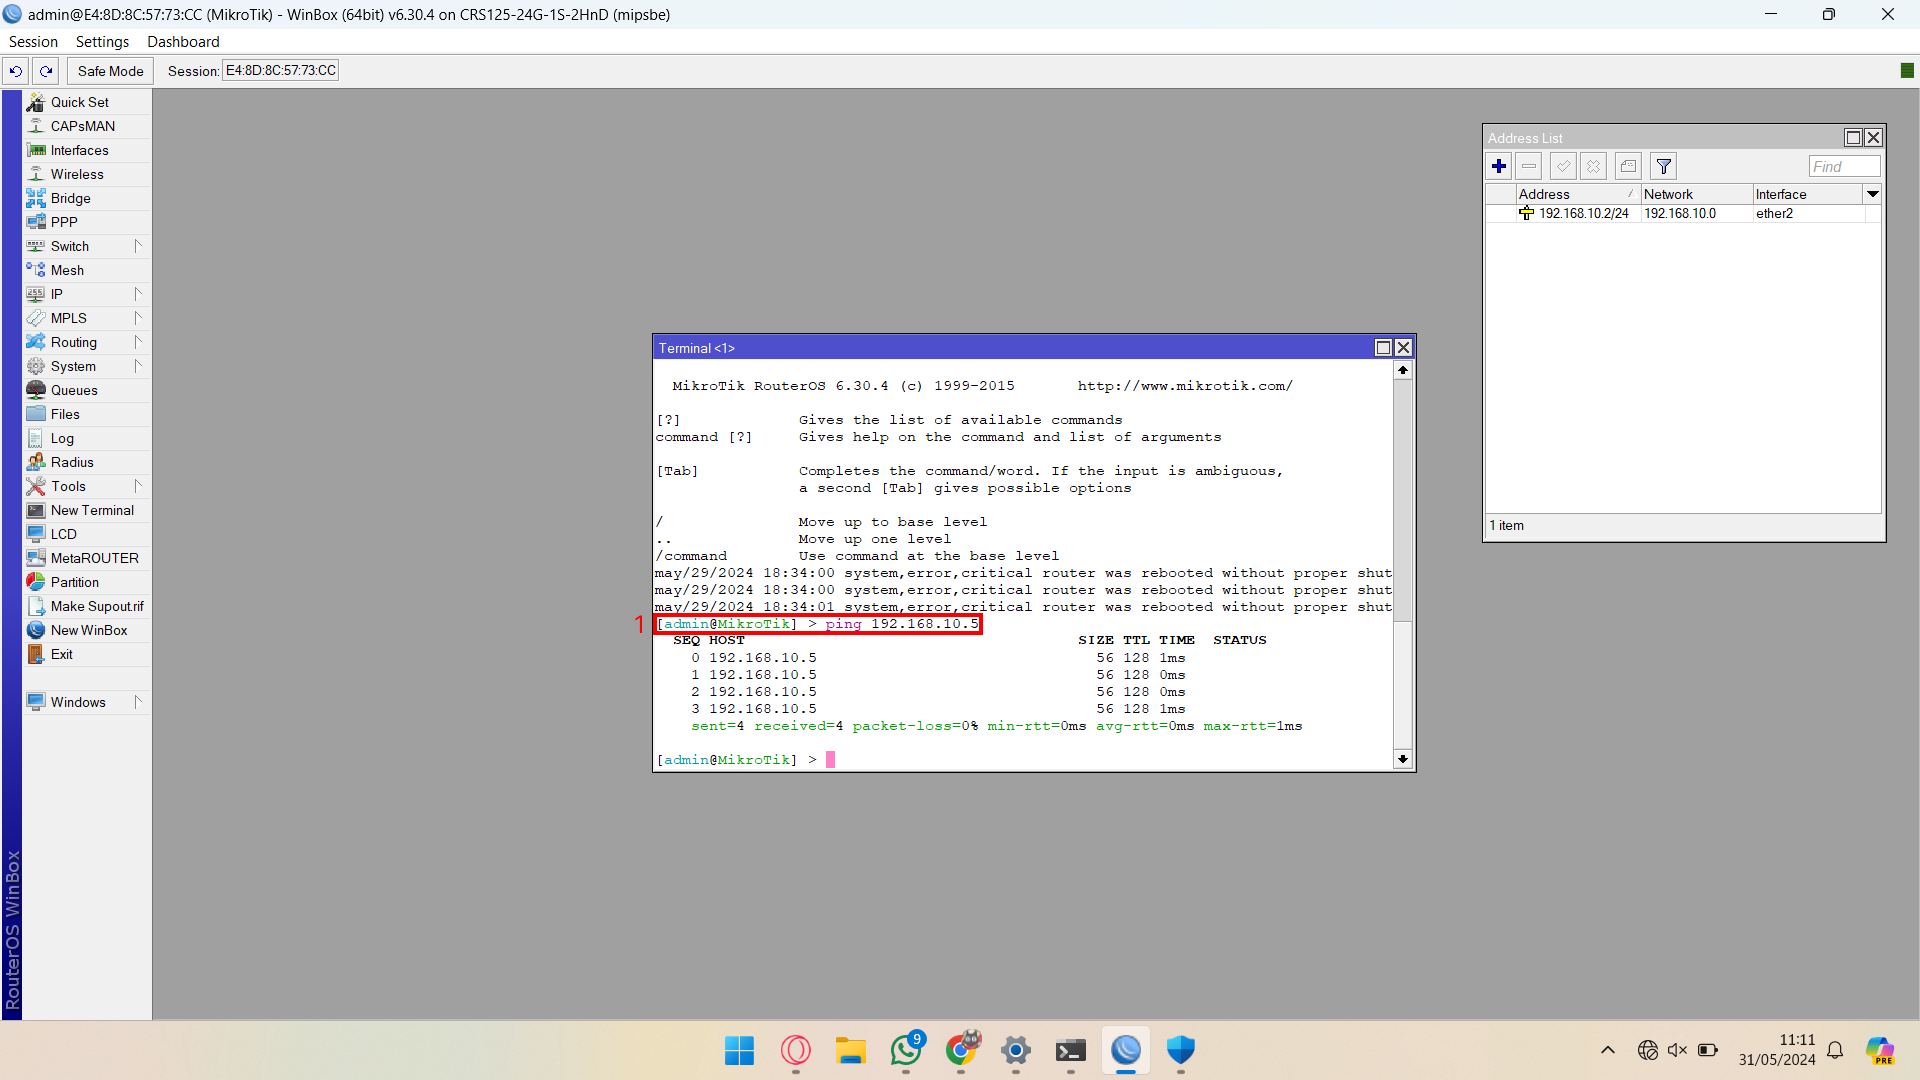
\includegraphics[width=0.8\linewidth]{P4/img/pc1/Step 5.png}
			\caption{Step 5}
			\label{fig:Step 5(PC 1)}
		\end{figure}
        \item Lakukan tes ping ke alamat Remote Address Router 2 untuk memastikan kedua Router sudah terhubung.
        \begin{figure}[H]
			\centering
			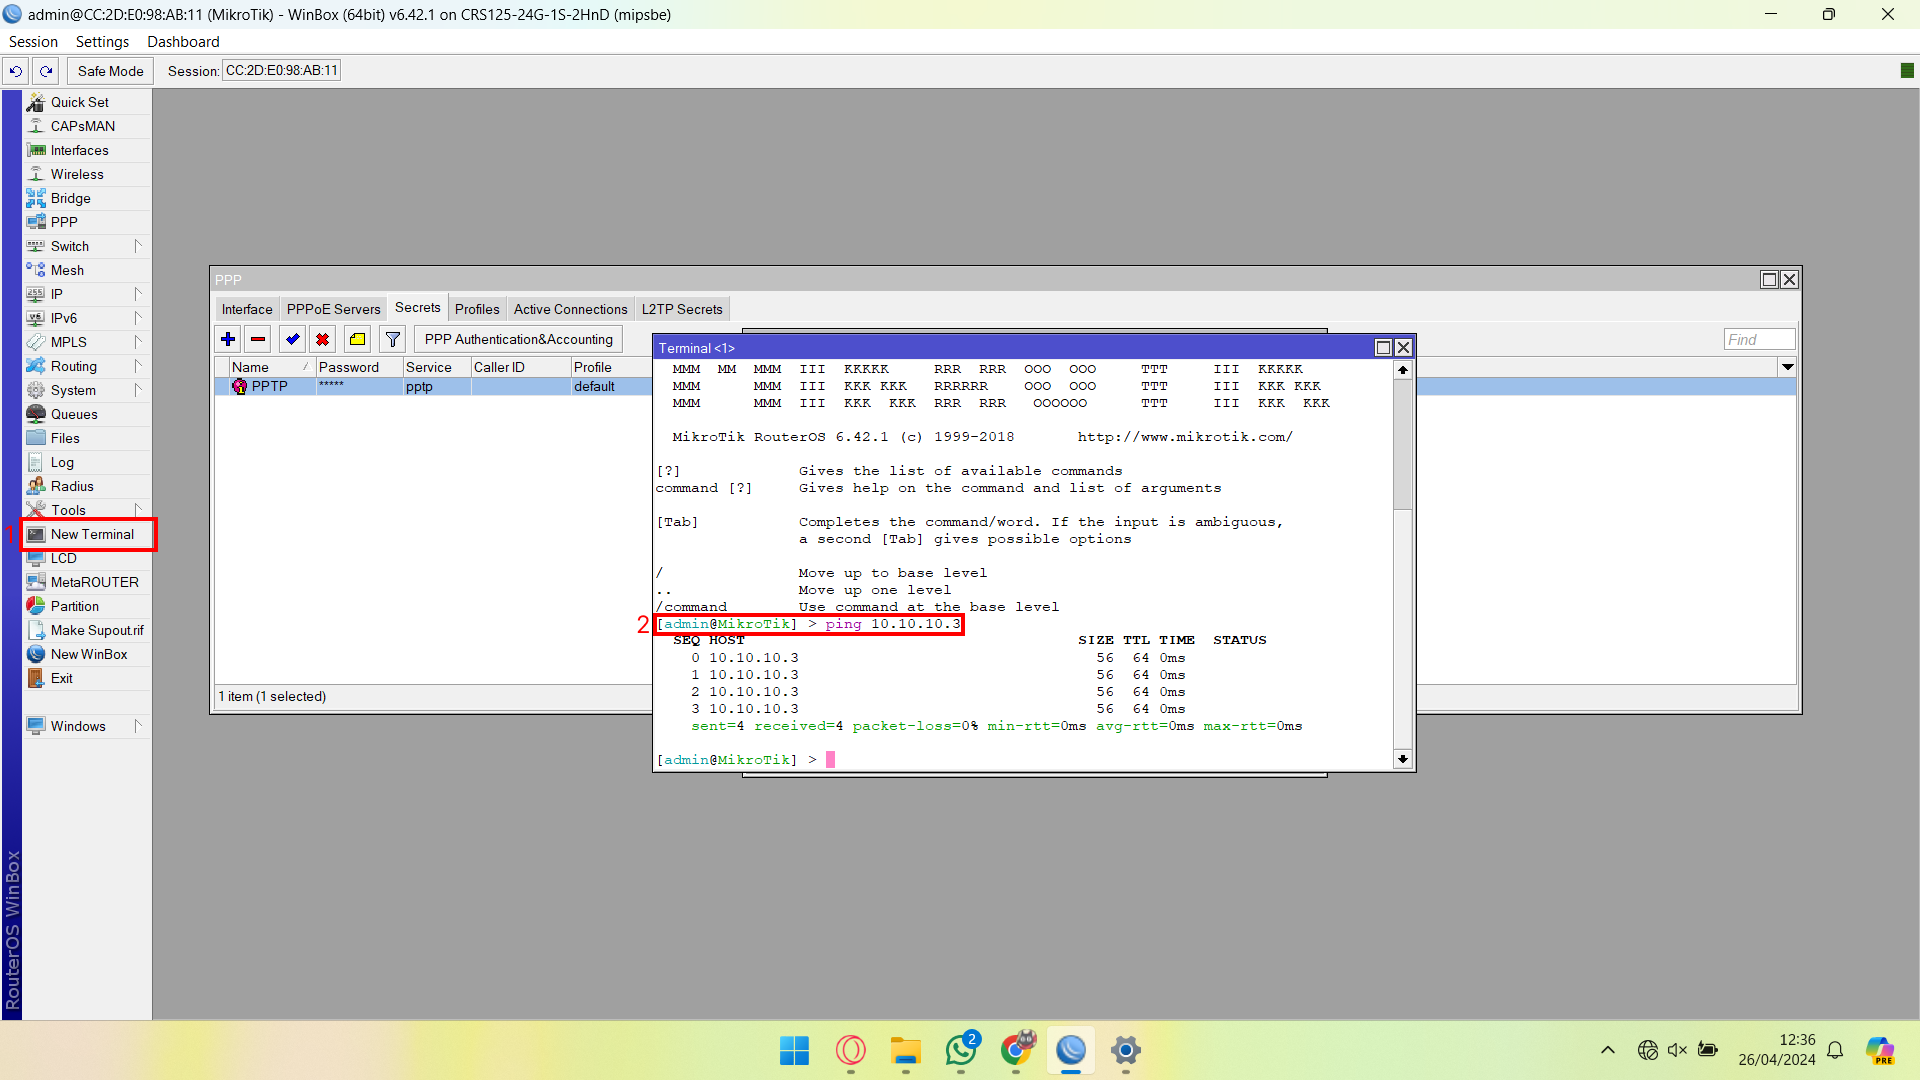
\includegraphics[width=0.8\linewidth]{P4/img/pc1/Step 5.1.png}
			\caption{Step 6}
			\label{fig:Step 6(PC 1)}
		\end{figure}
        \item Lakukan routing statis agar kedua PC dapat berkomunikasi. Buka pada tab IP > Routes, lalu tambahkan jaringan. Masukkan alamat jaringan yang ingin dituju, melalui alamat Gateway pada router 2
        \begin{figure}[H]
			\centering
			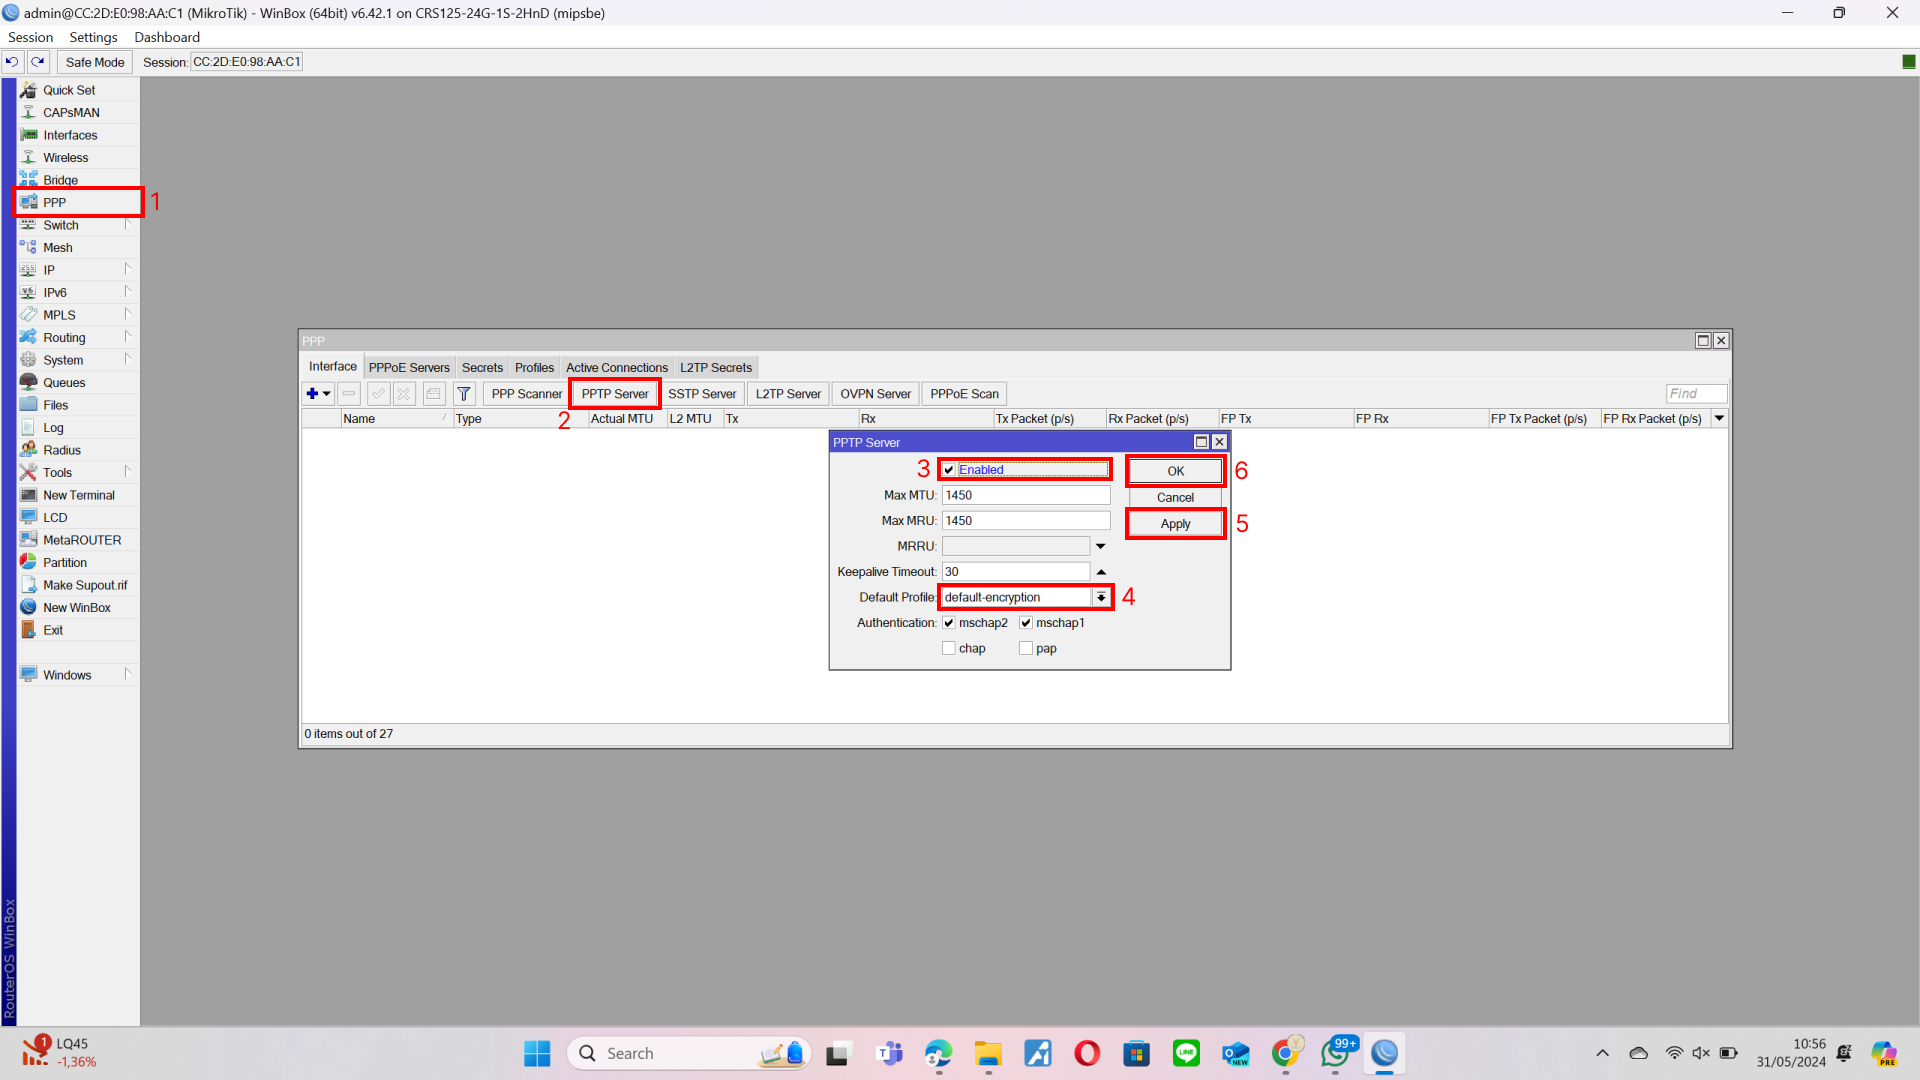
\includegraphics[width=0.8\linewidth]{P4/img/pc1/Step 6.png}
			\caption{Step 7}
			\label{fig:Step 7(PC 1)}
		\end{figure}
        \item Lakukan tes ping ke ke PC 2 untuk memastikan kedua PC sudah terhubung.
        \begin{figure}[H]
			\centering
			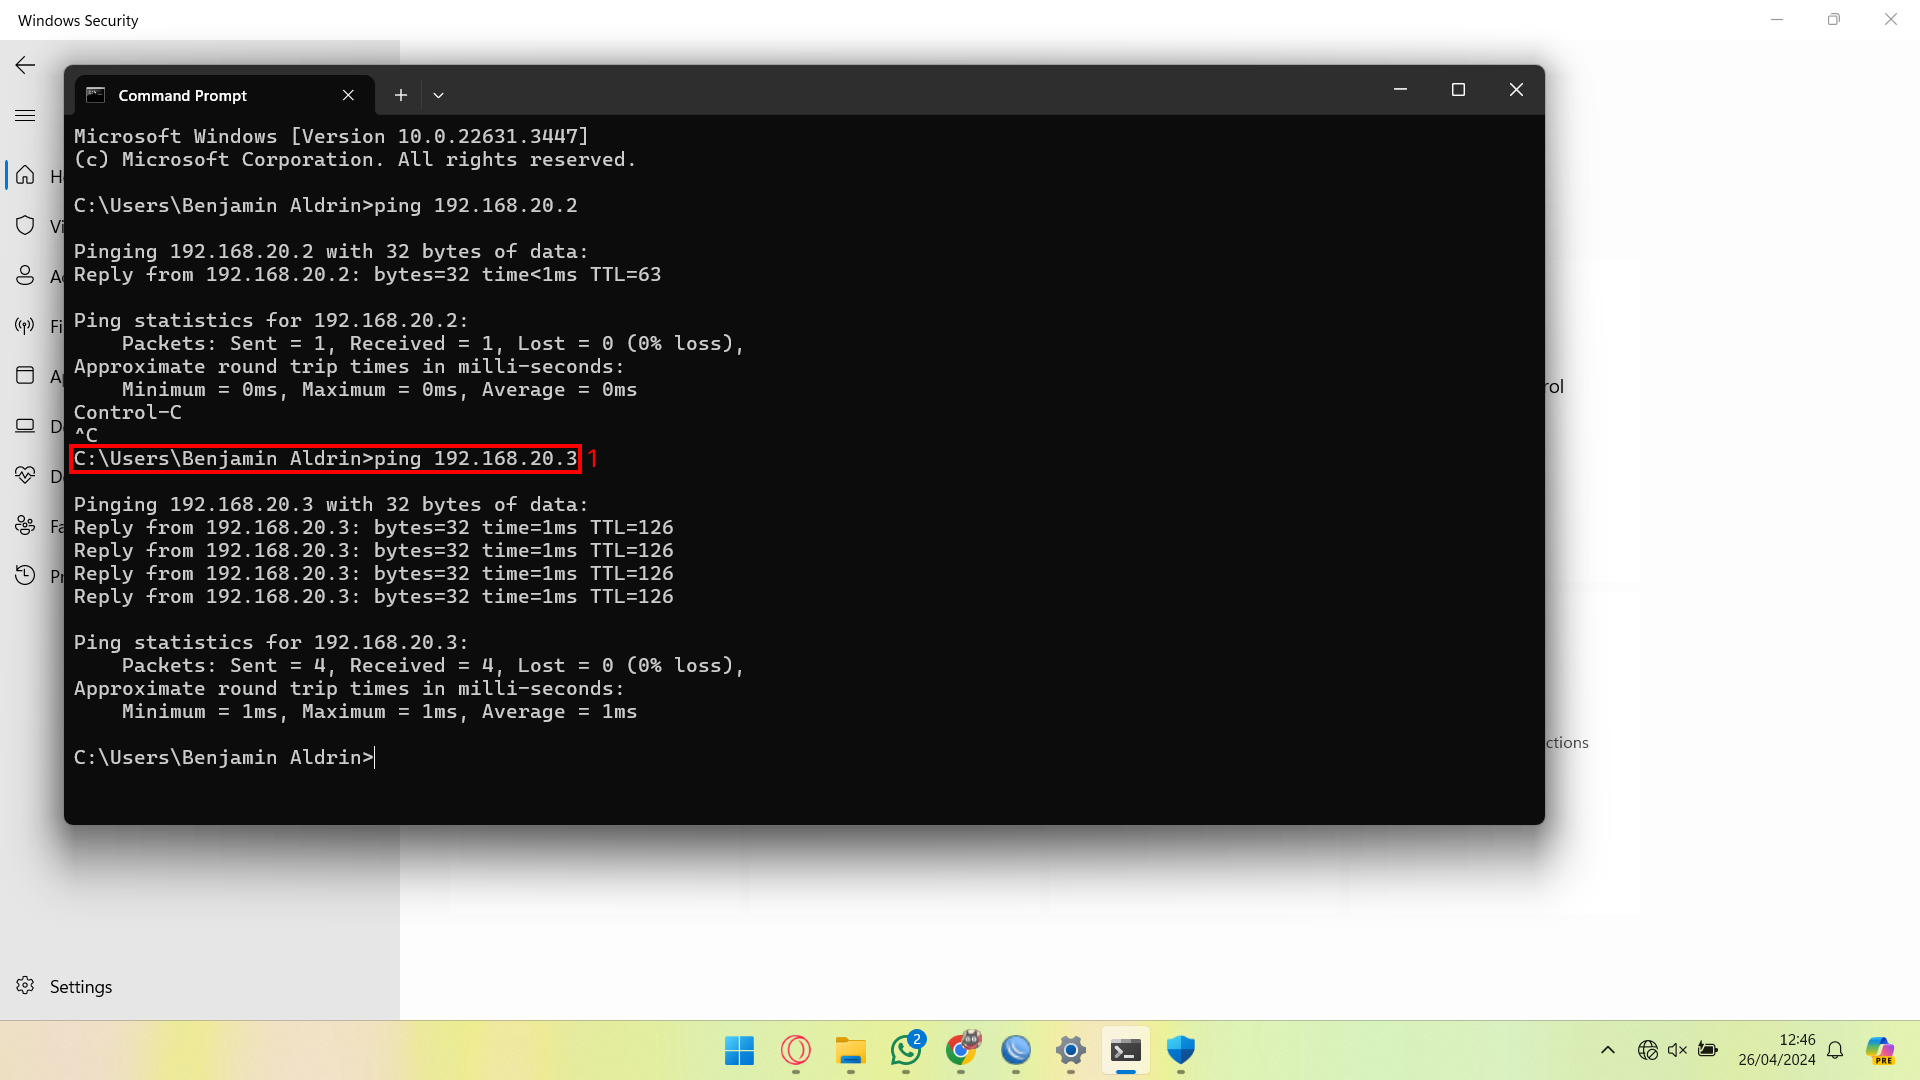
\includegraphics[width=0.8\linewidth]{P4/img/pc1/Step 7.png}
			\caption{Step 8}
			\label{fig:Step 8(PC 1)}
		\end{figure}
    \end{enumerate}

    \textbf{Konfigurasi PC 2}
    \begin{enumerate}
        \item Buka aplikasi Winbox pada PC dan lakukan hubungkan ke Router. Pastikan Login terisi “admin”, Klik Neighbors > Klik Refresh > Pilih Router yang ingin disambungkan > Klik Connect.
        \begin{figure}[H]
			\centering
			\includegraphics[width=0.5\linewidth]{P4/img/pc2/Step 1.png}
			\caption{Step 1}
			\label{fig:Step 1(PC 2)}
		\end{figure}
        \item Jadikan Router menjadi DHCP Client agar bisa mendapat IP address dari Internet ITS. IP > Klik DHCP Client > Tambahkan DHCP Client > Pilih interface yang terhubung dengan Internet (ether2)> Klik Apply > Klik OK. Kita bisa memastikan koneksi ke internet dengan cara melakukan tes ping ke alamat IP 8.8.8.8
        \begin{figure}[H]
			\centering
			\includegraphics[width=0.5\linewidth]{P4/img/pc2/Step 2.1.png}
			\caption{Step 2.1}
			\label{fig:Step 2.1(PC 2)}
        \end{figure}
        \begin{figure}[H]
			\centering
			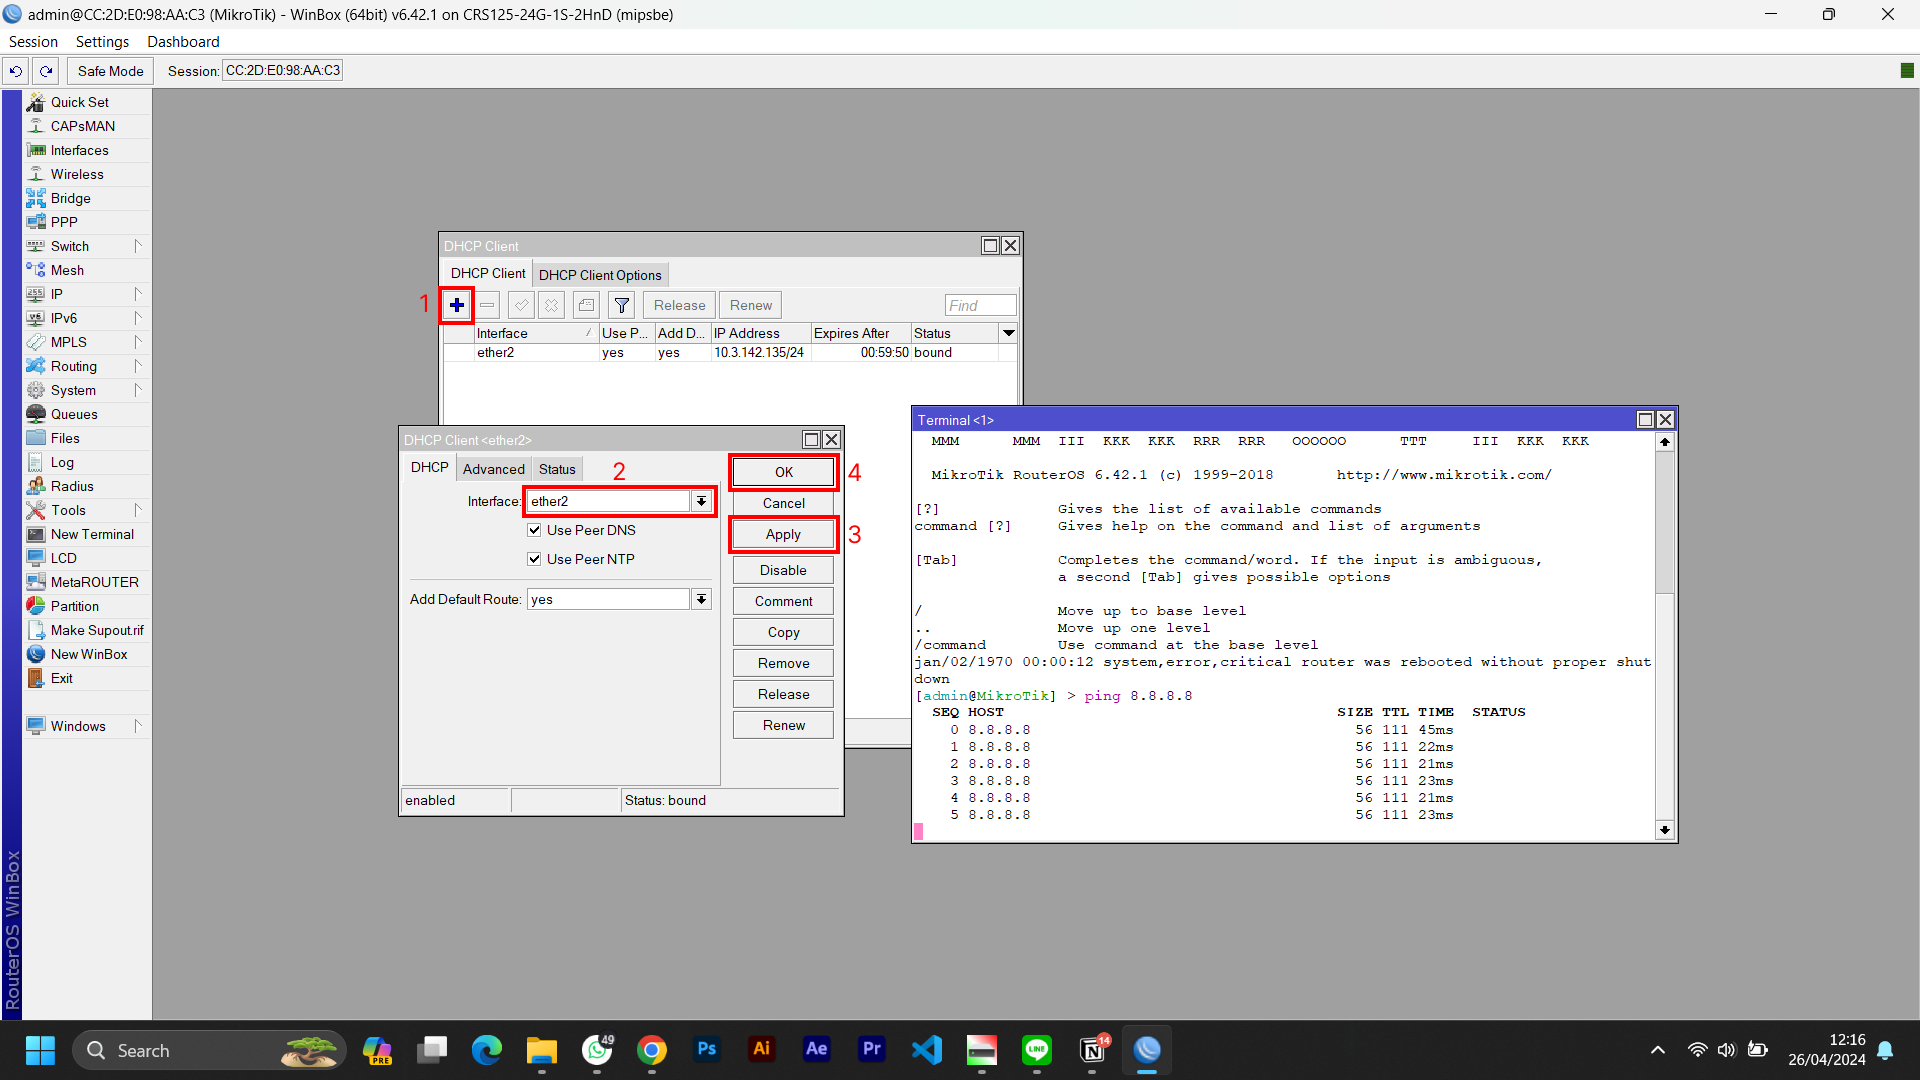
\includegraphics[width=0.8\linewidth]{P4/img/pc2/Step 2.2.png}
			\caption{Step 2.2}
			\label{fig:Step 2.2(PC 2)}
		\end{figure}
        \item Buat IP address baru pada Router 2 untuk menghubungkan PC 2 dengan Router 2. Tambahkan IP address > Isi address > Pilih Interface yang terhubung ke PC (ether4) > Klik Apply > Klik OK.
        \begin{figure}[H]
			\centering
			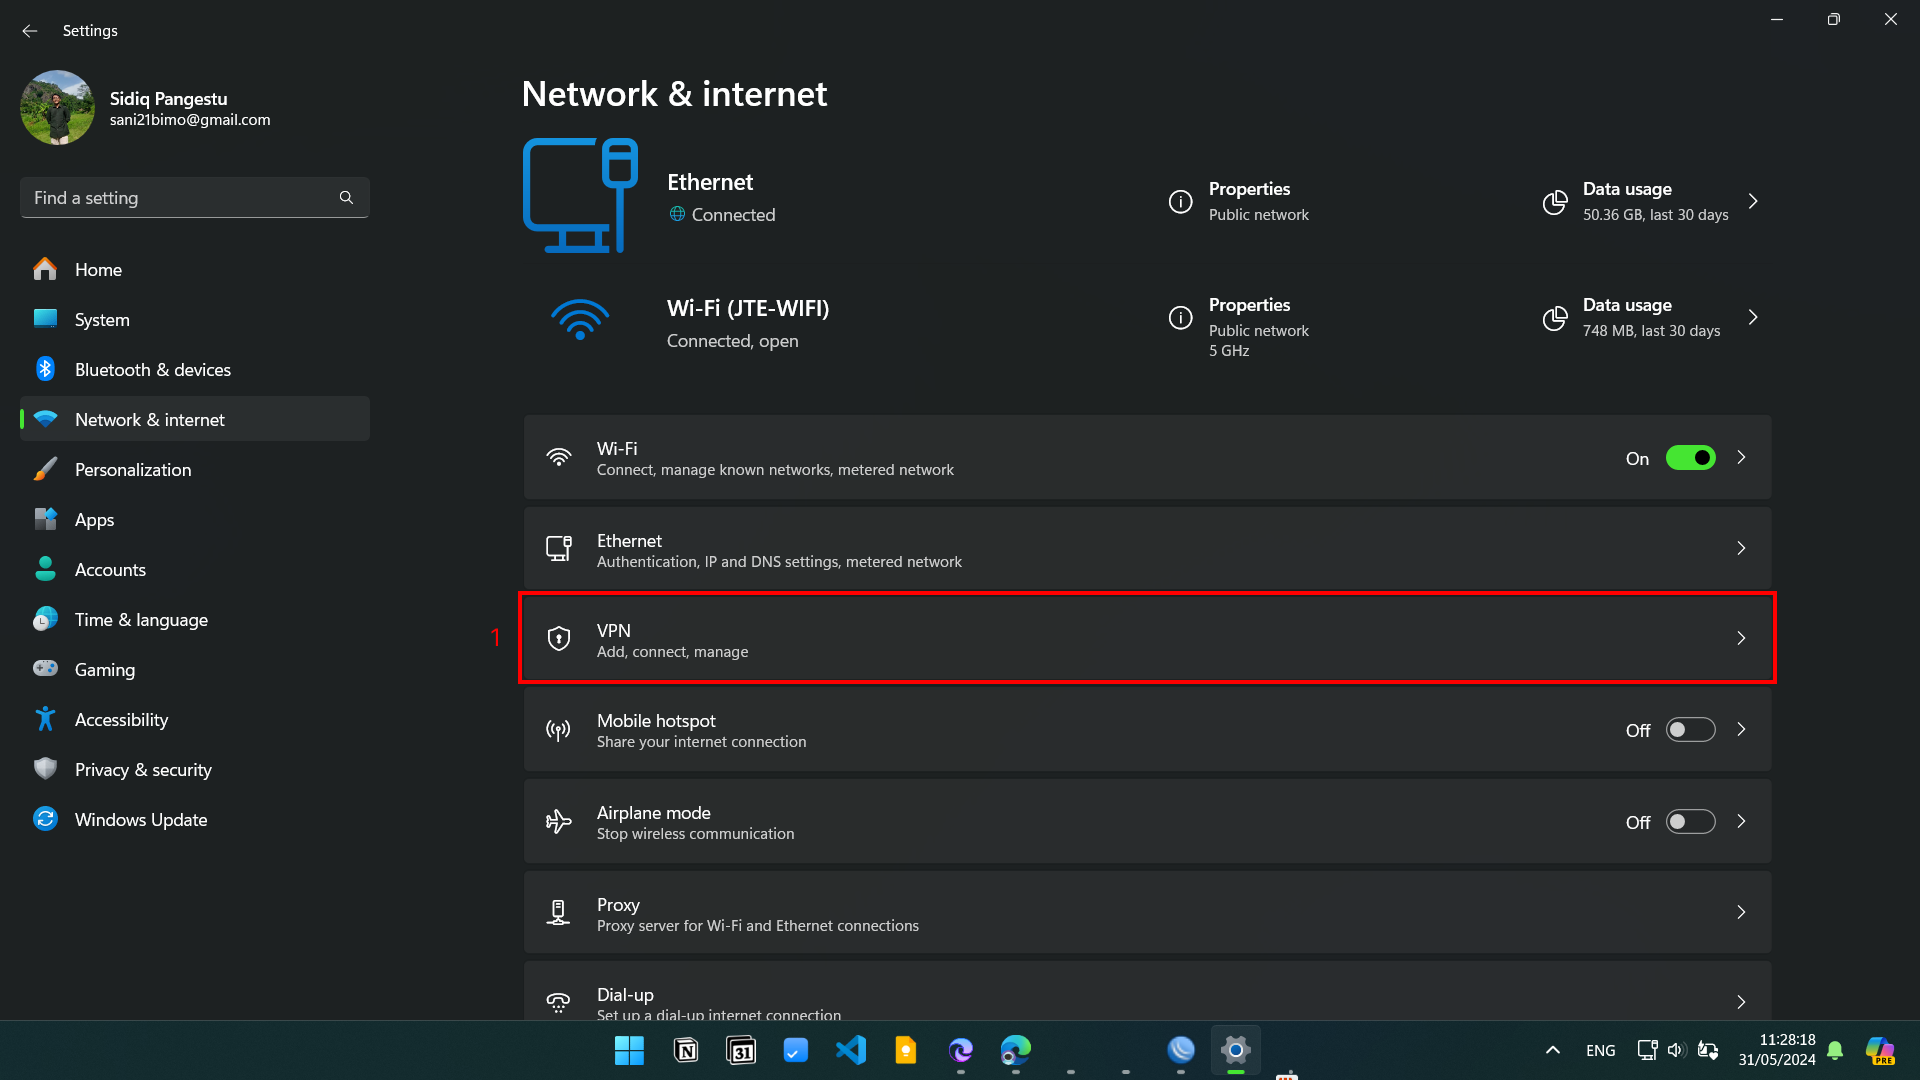
\includegraphics[width=0.8\linewidth]{P4/img/pc2/Step 3.png}
			\caption{Step 3}
			\label{fig:Step 3(PC 2)}
		\end{figure}
        \item Atur IP pada PC 2 dengan mengubah pengaturan pada setting ethernet. Ubah IP perangkat yang otomatis menjadi manual, pastikan IP PC 2 masih satu jaringan dengan IP lokal yang diinginkan, isi Gateway dengan IP address Router 2 yang tersambung dengan PC 2. Berikan IP address yang berbeda dengan contoh yang ada di modul.
        \begin{figure}[H]
			\centering
			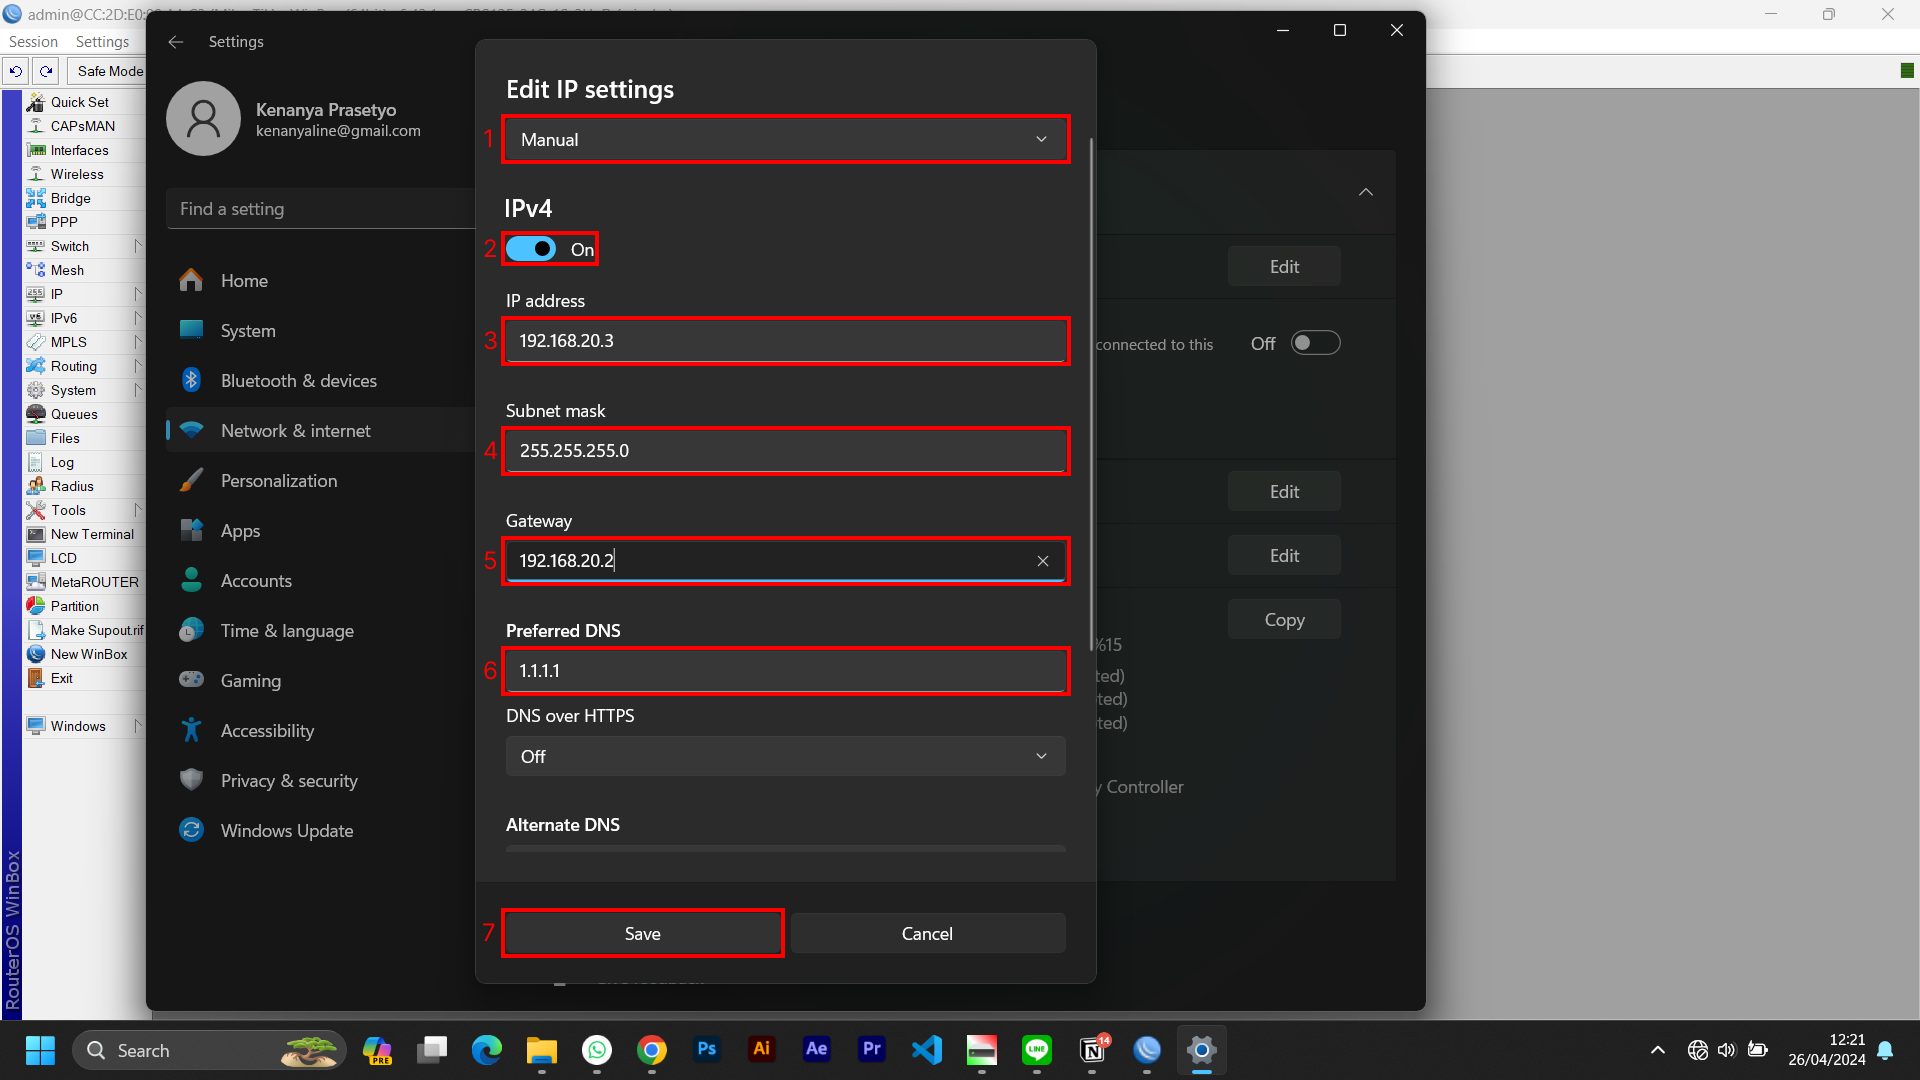
\includegraphics[width=0.8\linewidth]{P4/img/pc2/Step 4.png}
			\caption{Step 4}
			\label{fig:Step 4(PC 2)}
		\end{figure}
        \item Hubungkan client PPTP dengan server PPTP, untuk melakukan hal tersebut, buatlah PPTP Client baru kemudian konfigurasi koneksi pada tab Dial Out, dengan konfigurasi Connect To “10.3.142.134”, Connect To adalah IP address pada Router 1 yang terhubung ke internet. konfigurasi Nama “PPTP”, Password “123456”, Profile “default-encryption”. Pastikan Nama dan Password sesuai dengan yang sudah di buat.
        \begin{figure}[H]
			\centering
			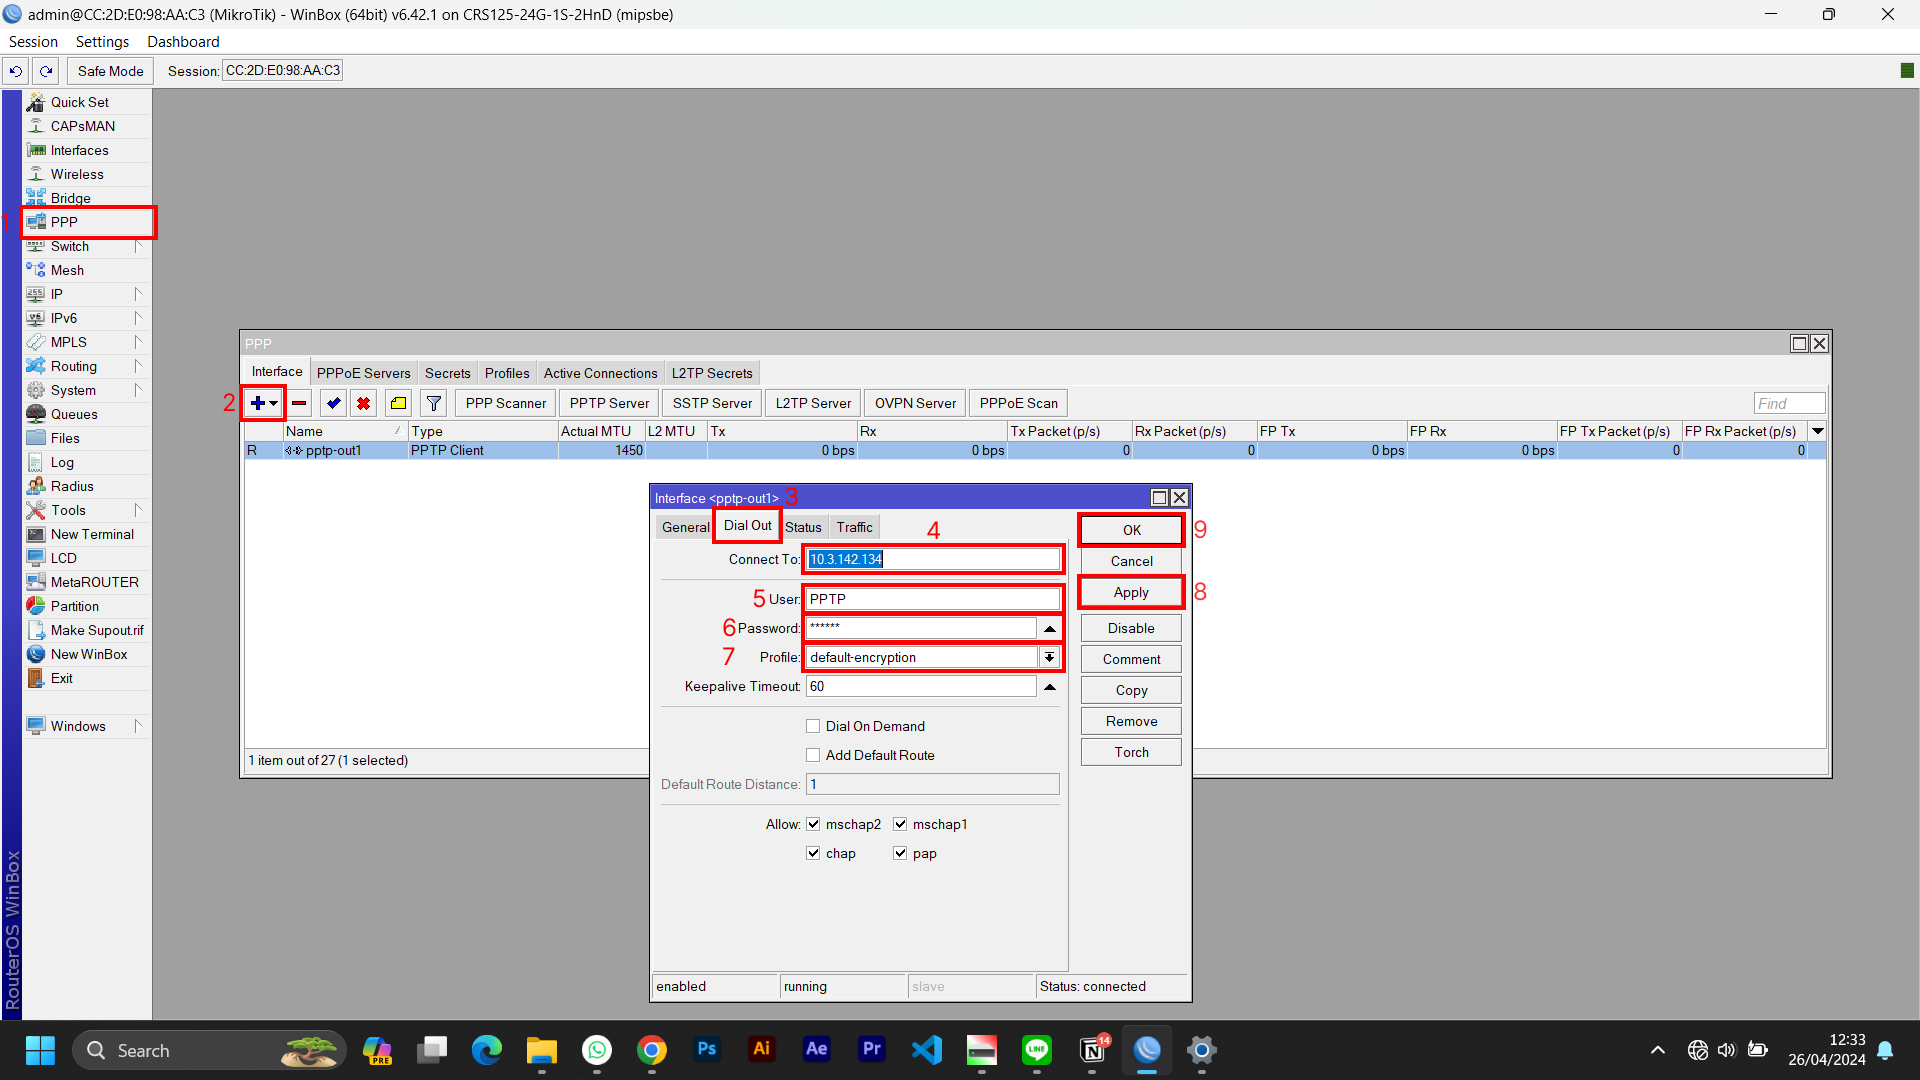
\includegraphics[width=0.8\linewidth]{P4/img/pc2/Step 5.png}
			\caption{Step 5}
			\label{fig:Step 5(PC 2)}
		\end{figure}
        \item Lakukan tes ping ke alamat Local Address Router 1 untuk memastikan kedua Router sudah terhubung.
        \begin{figure}[H]
			\centering
			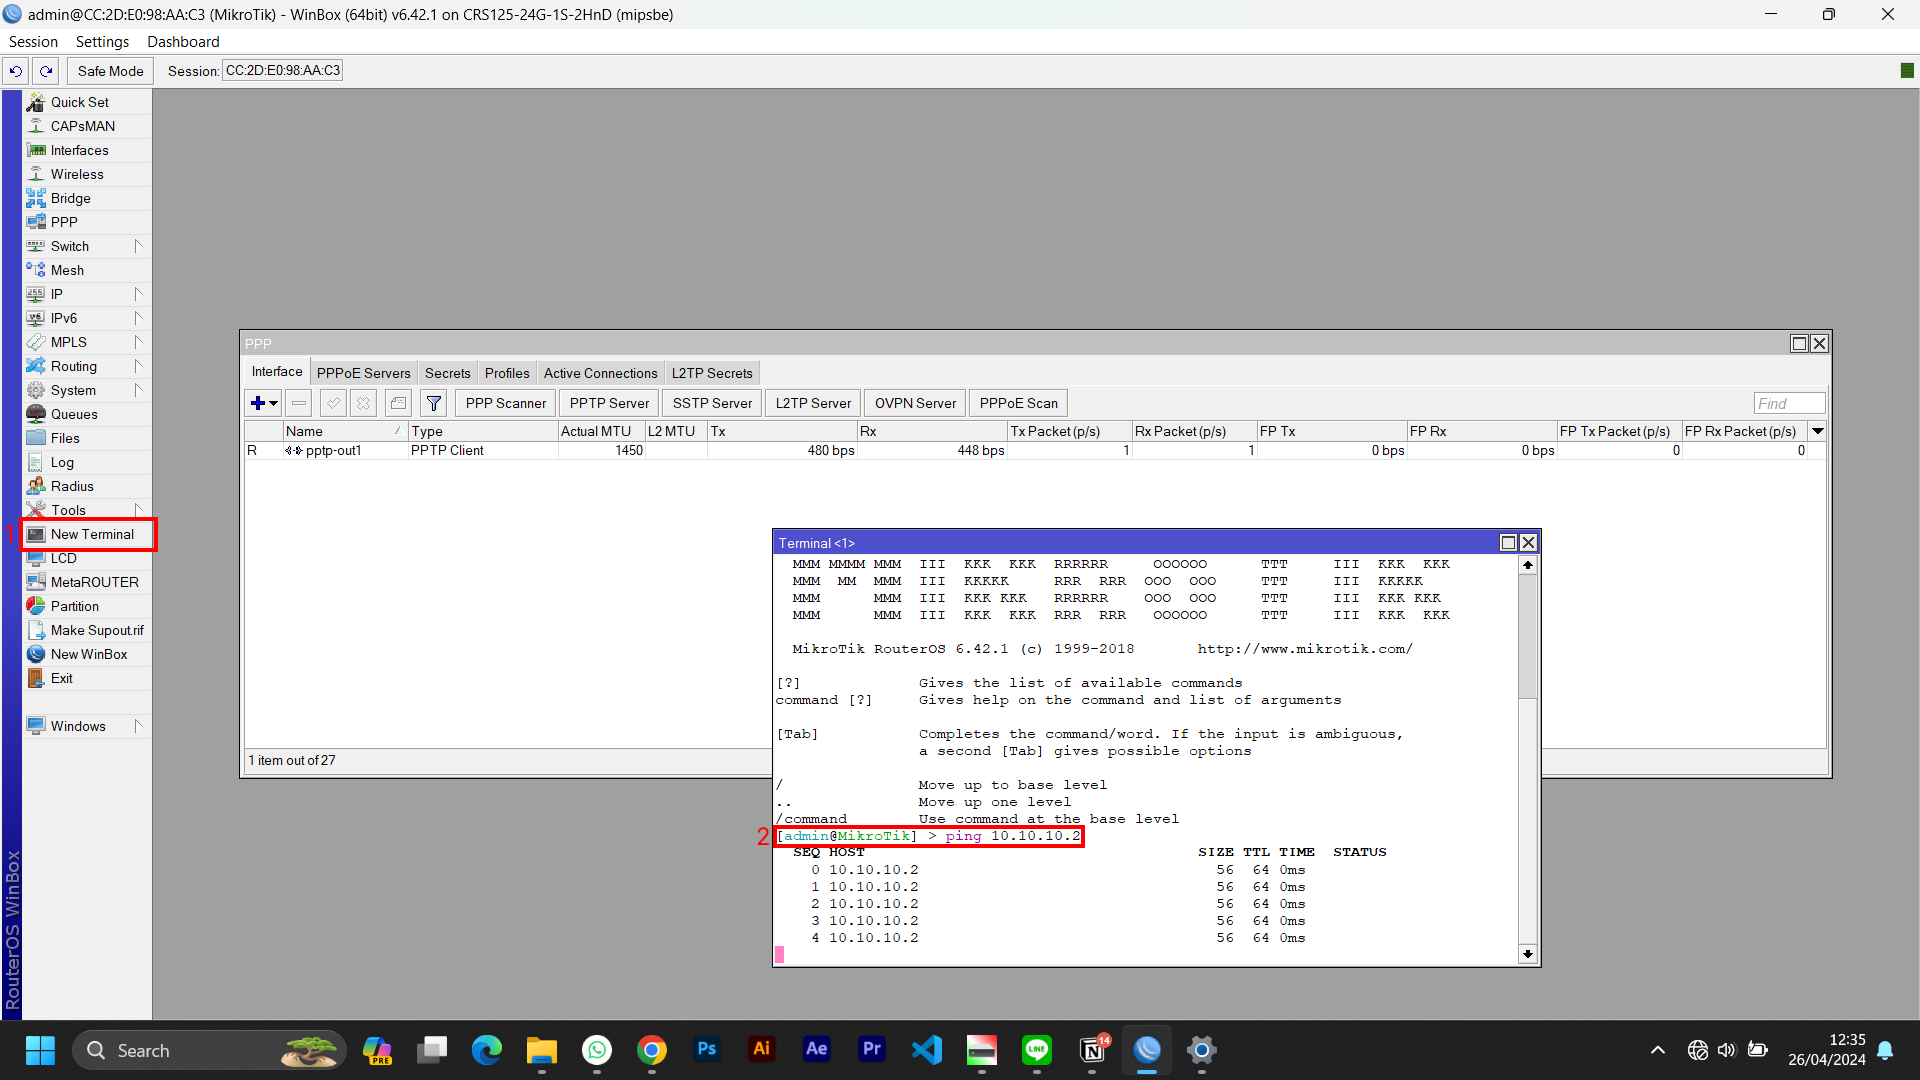
\includegraphics[width=0.8\linewidth]{P4/img/pc2/Step 5.1.png}
			\caption{Step 6}
			\label{fig:Step 6(PC 2)}
		\end{figure}
        \item Lakukan routing statis agar kedua PC dapat berkomunikasi. Buka pada tab IP > Routes, lalu tambahkan jaringan. Masukkan alamat jaringan yang ingin dituju, melalui alamat Gateway pada router 2
        \begin{figure}[H]
			\centering
			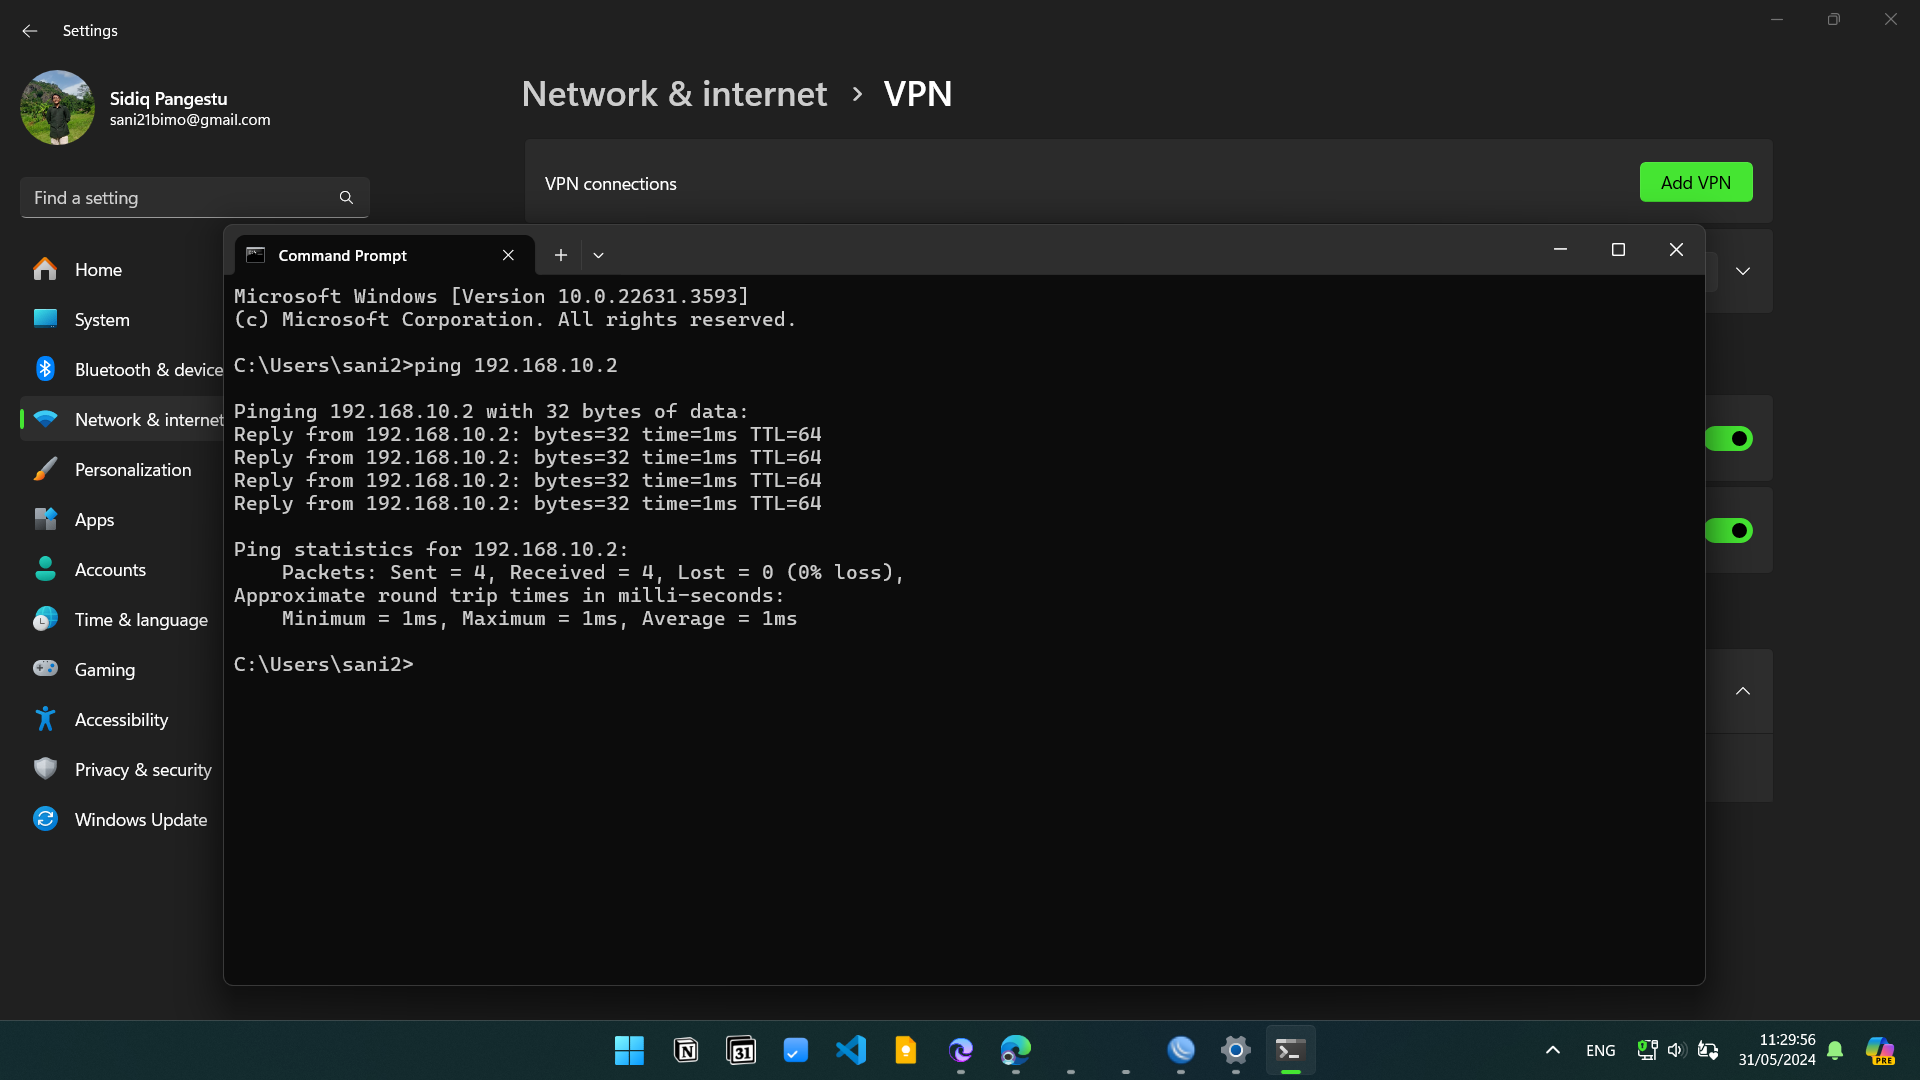
\includegraphics[width=0.8\linewidth]{P4/img/pc2/Step 6.png}
			\caption{Step 7}
			\label{fig:Step 7(PC 2)}
		\end{figure}
        \item Lakukan tes ping ke ke PC 1 untuk memastikan kedua PC sudah terhubung.
        \begin{figure}[H]
			\centering
			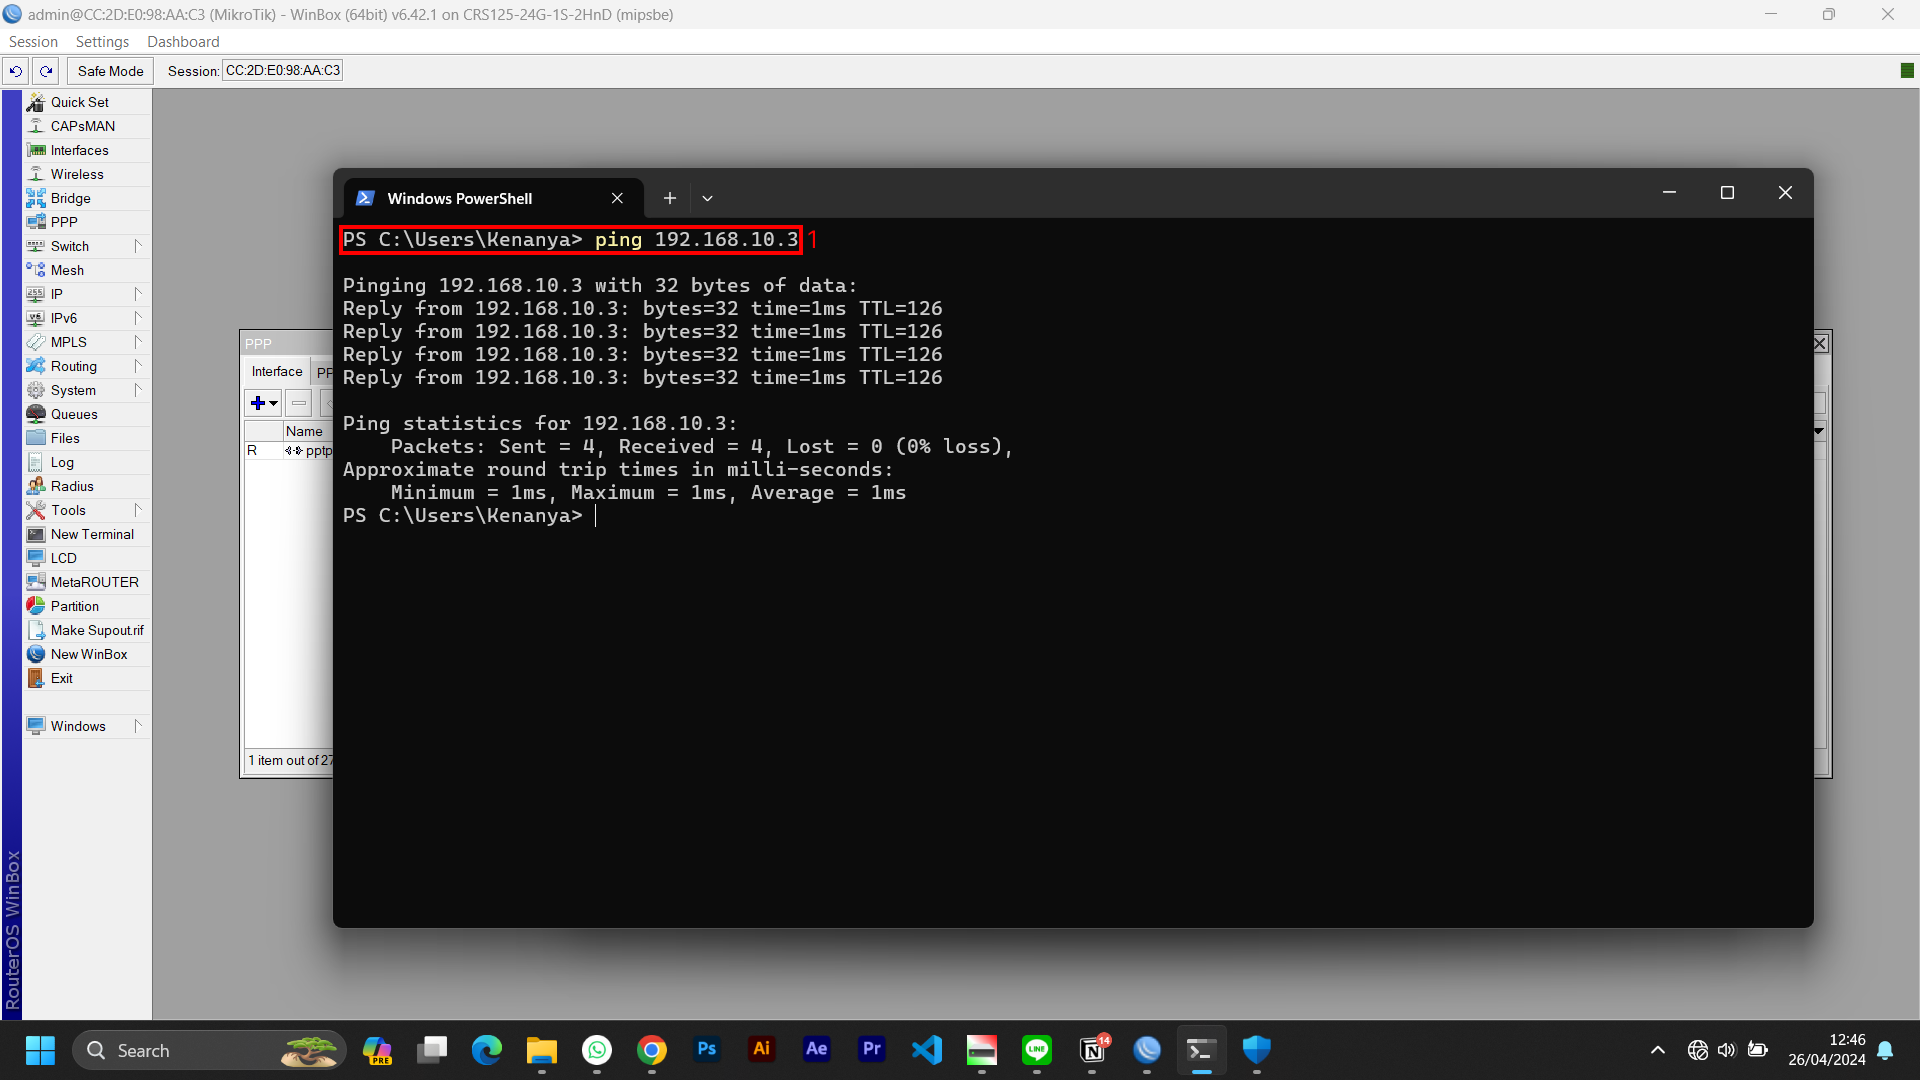
\includegraphics[width=0.8\linewidth]{P4/img/pc2/Step 7.png}
			\caption{Step 8}
			\label{fig:Step 8(PC 2)}
		\end{figure}
    \end{enumerate}
\end{center}

%===========================================================%
\section{Hasil yang didapat}
Memahami penerapan dan penghubungan jaringan dengan menerapkan PPTP dengan VPN

%===========================================================%
\section{Kesimpulan}
Dalam mengkonfigurasi VPN, diperlukan pemahaman dasar mengenai metode PPTP, dan juga diperlukan ketelitian dan fokus agar berhasil
